\documentclass[a4paper, 12pt]{report}
\usepackage[utf8]{inputenc}
\usepackage[T1]{fontenc}

\usepackage{xcolor}
\usepackage{afterpage}

\usepackage{relsize}
\usepackage{moresize}

\usepackage{graphicx}
\usepackage{geometry}

\usepackage{hyperref}
\usepackage{apacite}

\usepackage{amsmath}
\usepackage{amssymb}

\usepackage{caption}
\usepackage{subcaption}

\setcounter{secnumdepth}{3}
\setcounter{tocdepth}{3}

% [CHANGE] The title of your thesis. If your thesis has a subtitle, then this
% should appear right below the main title, in a smaller font.
\newcommand{\theTitle}{The first sentence \\
\vspace{0.5em}
the second sentence}
\newcommand{\theSubTitle}{a smaller subtitle}


% [CHANGE] Your full name. In case of multiple names, you can include their
% initials as well, e.g. "Robin G.J. van Achteren".
\newcommand{\theAuthor}{Dewi E. Timman}

% [CHANGE] Your student ID, as this has been assigned to you by the UvA
% administration.
\newcommand{\theStudentID}{12419273}

% [CHANGE] The name of your supervisor(s). Include the titles of your supervisor(s),
% as well as the initials for *all* of his/her first names.
\newcommand{\theSupervisor}{Dr. V. Niculae} % Dr. Ing. L. Dorst

% [CHANGE] The address of the institute at which your supervisor is working.
% Be sure to include (1) institute (is appropriate), (2) faculty (if
% appropriate), (3) organisation name, (4) organisation address (2 lines).
\newcommand{\theInstitute}{
Informatics Institute \\ %Institute for Logic, Language and Computation
Faculty of Science\\
University of Amsterdam\\
Science Park 900 \\ 
1098 XH Amsterdam 
}

% [CHANGE] The semester in which you started your thesis.
\newcommand{\theDate}{Semester 1, 2023-2024}

\begin{document}
\pagestyle{empty}
\begin{center}

\vspace{2.5cm}


\begin{Huge}
% see definition at beginning of document
\theTitle
\end{Huge} \\

\vspace{0.5 cm}

\begin{Large}
\theSubTitle
\end{Large}

\vspace{1.5cm}

% see definition at beginning of document
\theAuthor\\
% see definition at beginning of document
\theStudentID

\vspace{1.5cm}

% [DO NOT CHANGE]
Bachelor thesis\\
Credits: 18 EC

\vspace{0.5cm}

% [DO NOT CHANGE] The name of the educational programme.
Bachelor \textit{Kunstmatige Intelligentie} \\
\vspace{0.25cm}

\includegraphics[width=0.075\paperwidth]{figs/uva_logo} \\
\vspace{0.1cm}

% [DO NOT CHANGE] The address of the educational programme.
University of Amsterdam\\
Faculty of Science\\
Science Park 900\\
1098 XH Amsterdam

\vspace{2cm}

\emph{Supervisor}\\

% see definition at beginning of document
\theSupervisor

\vspace{0.25cm}

% see definition at beginning of document
\theInstitute

\vspace{1.0cm}

% see definition at beginning of document
\theDate

\end{center}
\newpage

\pagenumbering{arabic}
\setcounter{page}{1}
\pagestyle{plain} 

\chapter*{Abstract}
% TODO
\textbf{keywords:} 

\tableofcontents

\chapter{Introduction}
% What am I researching? bruggetje met taal
% \begin{itemize}
%     \item keywords $\rightarrow$ sentence
%     \item efficient, accurate, interpretable
%     \item this research: segmentation model more effective, natural, flexible than a bit mask?
% \end{itemize}

What if machines can read our mind? 
If we can give a machine a few keywords and let the machine generate a sentence from these keywords, our lives would become more productive and efficient. 
This is what autocomplete systems are trying to achieve. 
\textcolor{orange}{The way in which we choose the keywords is also important. 
Taking just the first or the last few words of a sentence as keywords usually does not capture the full meaning of the sentence.} 
For example, if someone want to capture the meaning of \textit{'I live in Amsterdam'} in a few keywords, the words \textit{'live Amsterdam'} would probably be choosen. 
Thus, the keywords come from multiple places in the sentence. 
Therefore, autocomplete systems need to use more complex models to be more efficient and accurate. 

\section{Literature review}
% TODO/delete

\subsection{Autocomplete communication game}

\begin{figure}
    \centering
    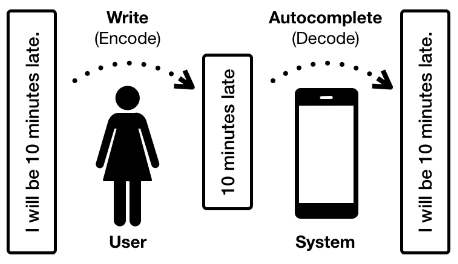
\includegraphics[width=.5\linewidth]{figs/autocomplete_game.png}
    \caption{schematic overview of the communication game. Figure from \protect\citeA{autocomplete}.}
    \label{fig:autocomplete}
\end{figure}

The same autocomplete communication game is considered as in \citeA{autocomplete}. In this game, a human (called user) encodes a sentence into keywords. 
These keywords are then decoded by a machine (called system) to retrieve the full, initial sentence. 
A schematic overview is given in figure \ref{fig:autocomplete}. 
The communication game is succesfull if the retrieved sentence is the same as the initial sentence. 

More formally, a target sentence $x=(x_1, \dots, x_m)$ is communicated by a user through the keywords $z=(z_1, \dots, z_n)$. 
Note that $z$ is a subsequence of $x$. 
The system then tries to retrieve the target sentence by decoding the keywords. 
The target sentence is described by the keywords using encoding strategy $q_{\alpha}(z | x)$ and the system decodes the keywords by using decoding strategy $p_{\beta}(x|z)$. 

For a model to be efficient, the number of keywords needs to be as low as possible. 
In addition, for a model to be accurate, the probability of reconstructing $x$ from $z$ needs to be as high as possible. 
Therefore, a cost and a loss, respectively, can be defined:
\begin{equation}
    \text{cost}(x,\alpha) = \mathbb{E}_{q_{\alpha}(z|x)} [\text{length}(z)]
\end{equation}
\begin{equation}
    \text{loss}(x,\alpha,\beta) = \mathbb{E}_{q_{\alpha}(z|x)} [-\log p_{\beta}(x|z)]
\end{equation}

\subsection{Segmentation model}
% Why does a segmentation model work?
% TODO: better captions for images
% TODO: add references
% TODO: add Markov Models

\subsubsection{General idea}
\textcolor{orange}{With a segmentation model all possible segmentation can be made. 
A segmentation model scores every possible segmentation.
With these scores, the model can determine what the best possible segmentation is.}

\subsubsection{Segmentation model for text}
So how does the segmentation model work for text? 
If we have a sentence, e.g. \textit{'I will be late'}, we can use fencepost indexing and represent the fenceposts as nodes in a directed acyclic graph (DAG). 
We can then draw edges between those nodes that represent segments. 
Those segments can be seen as (groups of) words. 
In figure \ref{fig:dag}, a DAG can be seen in which all the possible segments are showed. 
In the case of the autocomplete communication model described before, a segment is either kept or not.
Therefore, we can have one edge representing 'keep' and one representing 'do not keep', resulting in figure \ref{fig:dag2}.
If the pink edges are taken as 'do not keep' and the blue ones as 'keep', two possible segmentations can be seen in figure \ref{fig:segmentation} and \ref{fig:segmentation2}. 
Both segmentations result in the keywords \textit{'will be late'}. 

\begin{figure}
    \centering
    \begin{subfigure}[b]{0.45\textwidth}
        \centering
        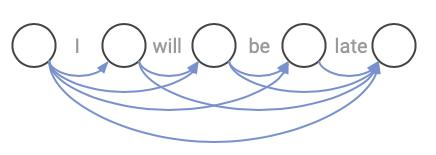
\includegraphics[width=\textwidth]{figs/segmentation1.jpeg}
        \caption{Segments as a DAG}
        \label{fig:dag}
    \end{subfigure}
    \hfill
    \begin{subfigure}[b]{0.45\textwidth}
        \centering
        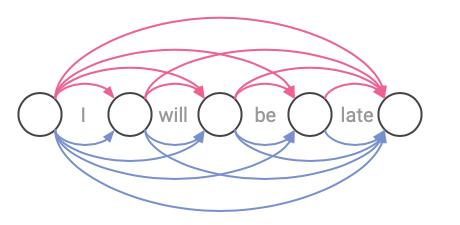
\includegraphics[width=\textwidth]{figs/segmentation2.jpeg}
        \caption{More segments as a DAG}
        \label{fig:dag2}
    \end{subfigure}
    \hfill
    \begin{subfigure}[b]{0.45\textwidth}
        \centering
        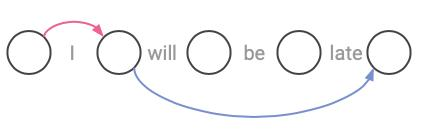
\includegraphics[width=\textwidth]{figs/segmentation3.jpeg}
        \caption{Possible segmentation}
        \label{fig:segmentation}
    \end{subfigure}
    \hfill
    \begin{subfigure}[b]{0.45\textwidth}
        \centering
        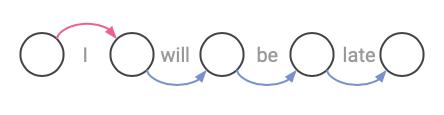
\includegraphics[width=\textwidth]{figs/segmentation4.jpeg}
        \caption{Another possible segmentation}
        \label{fig:segmentation2}
    \end{subfigure}
    \caption{Segmentation model.}
    \label{fig:segmentation_model}
\end{figure}

All segments can be scored with the help of the Forward algorithm. 
After scoring each segment, the model can then choose the segments with the highest scores to retrieve the best possible segmentation. 

\subsection{Structured latent variables}
How does the model work? 

\section{Current research}
% Gap
% Research question: To what extend can a segmentation model help by selecting keywords for an auto-complete communication game?

Previous research did not take structure into account \cite{autocomplete, Bar-YossefZiv2011Cqa, SvyatkovskiyAlexey2019PACC}.
Since language is structured, it makes sense to use a structured model as an autocomplete model. 
In this research, we look at how we can use a latent segmentation model to retrieve keywords from a sentence. 
The segmentation model will be implemented in the encoder of the encoder-decoder model in order to choose the best keywords from the sentence.

\chapter{Method}

\chapter{Results}

\chapter{Conclusion}

\chapter{Discussion}

\bibliography{articles.bib}
\bibliographystyle{apacite}

\end{document}